
\chapter{Residual Learning}
\label{app:residual}



\epigraph{No Doc\index{Brown, Emmett Lathrop ``Doc''}, not me, the other me! The one that's up on stage playing \neo{Johnny B. Goode}!}{Marty McFly \cite{BttFP2}.\index{McFly, Martin Seamus ``Marty''}}



\noindent{}In this final appendix, we'll analyze neural networks with residual connections\index{residual connection}, generally called  \textbf{residual networks}\index{residual network|textbf}.
These networks
were originally introduced in order to enable the training of deeper and deeper networks: traditionally deep networks suffer from the \neo{exploding and vanishing gradient problem}, but even in networks where various tricks of the trade are used to ensure the propagation of forward and backward signals, 
overly-deep\index{overly deep} 
networks are empirically found to have \emph{higher training and test errors} than their shallower-network counterparts.


From the \terminate{microscopic perspective}, 
 the increase of the 
\terminate{generalization error} is intuitive for a deeper model with more \terminate{model parameters}, but the increase in the training error is not: the additional parameters should naively enable \emph{better} fits to the training data.
At the very least, one might hope that the additional layers could 
-- in principle --
approximate the identity map and do \emph{no worse}.
Yet the empirical evidence mentioned above suggests that it's difficult for optimization algorithms 
to tune the
hidden layers of a deep network %
to such a nearly-identity map.
This is called \textbf{degradation}\index{degradation problem|textbf}\index{degradation problem|seealso{residual network}}\index{degradation problem|seealso{overly deep}}, and in principle 
is
a major limiting factor for developing larger scale deep-learning models.



From the \terminate{macroscopic perspective} of our effective theory, we can offer a \emph{dual}\index{duality!microscopic-macroscopic} explanation for this degradation problem.
As a precursor to our explanation, first recall that, rather than using any heuristic approach to solve the \terminate{exploding and vanishing gradient problem}, in \S\ref{sec:EVGP-WEP}
we analytically solved its \emph{exponential} manifestation by means of \terminate{criticality} and then solved its \emph{polynomial} manifestation by means of the learning-rate \terminate{equivalence principle}.
In \S\ref{sec:generalization-at-infinity} we further confirmed that the associated tunings of the \terminate{initialization hyperparameters}, $\Cb{\ell}$ and $\CW{\ell}$, and of the \terminate{training hyperparameters}, $\Lb{\ell}$ and $\LW{\ell}$,  lead to the most robust generalization performance for MLPs. 

Now, \emph{even if} these hyperparameters are  properly tuned, we would expect that overly-deep networks 
will suffer horribly from instantiation-to-instantiation \terminate{fluctuations}, leading to the breakdown of \terminate{criticality} for any \emph{particular} network. This problem was first discussed in \S\ref{sec:solution_DLN} for extremely deep (linear) networks, then more generally  in \S\ref{sec:signal_prop_finite_width}, and finally in footnote~\ref{footnote:epilogue-chaos} of Epilogue~\ref{epi:overparameterization}. Thus, combined with our discussion  
of the MLP's depth-to-width ratio $r\equiv L/n$ in 
\S\ref{sec:information-beyond-infinity},
perhaps we %
can understand the training loss degradation\index{degradation problem} problem in terms of the network leaving the regime of optimality and proceeding towards the regime of \terminate{chaos}.


If you'll please move the microscopic explanation back to the front of your mind, we can explain an ingenious solution to 
degradation
by He \emph{et al.}~\cite{he2016deep}.
Rather than trying to find a better learning algorithm, we can instead modify the deep network architecture so that the hidden layers 
only have to learn a \neo{residual function}: in place of a generic nonlinear $(\ell+1)$-th layer
\be\label{eq:zeroth-residual-connection}
z^{(\ell+1)}=\layer\!\le(z^{(\ell)}; \theta^{(\ell+1)}\ri)\, ,
\ee
we design the layer as
\be\label{eq:first-residual-connection}
z^{(\ell+1)}=\block\!\le(z^{(\ell)}; \theta^{(\ell+1)}\ri) + z^{(\ell)}\, ,
\ee
such that the \term{residual block}, $\block\!\le(z^{(\ell)}; \theta^{(\ell+1)}\ri)$,
is the residual of the function
that we want our layer, \eqref{eq:zeroth-residual-connection}, to implement.
The basic structure of this generic residual layer is depicted in the left panel of Figure~\ref{fig:residual-example} and will be further explained later on.


\begin{figure}
\begin{center}
 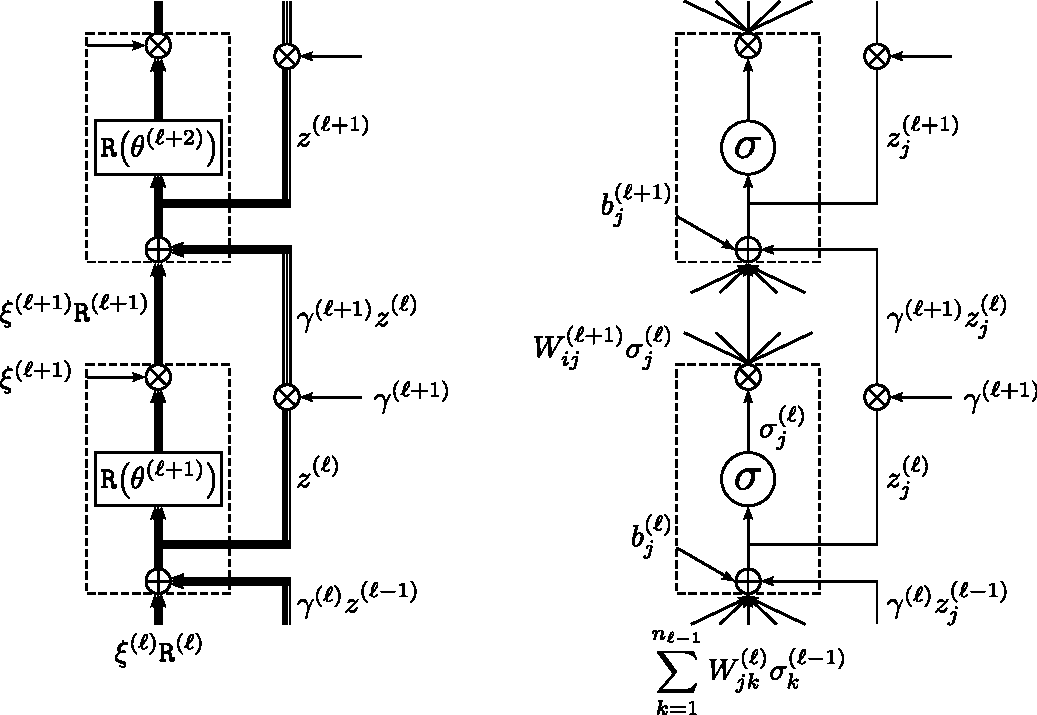
\includegraphics[width=1\linewidth]{./book_figures/residual.pdf}
\caption{
\textbf{Left:} two residual blocks\index{residual block} from adjacent layers for a very general \neo{residual network}. This detailed structure depicts how  each layer
\emph{(i)} adds a weighted block and the weighted preactivation to produce the next layer's preactivation,
\emph{(ii)} copies the preactivation to skip to the next layer,
and \emph{(iii)} generates the next layer's block.
\textbf{Right:} two neurons from adjacent layers for a 
\emph{residual MLP}.\index{multilayer perceptron!with residual connections} 
This detailed structure depicts how each layer \emph{(i)} adds the bias, 
the weighted activation, and the weighted preactivation 
to produce the next layer's preactivation, 
\emph{(ii)} copies the preactivation to skip to the next layer,
\emph{(iii)} generates the activation 
from the preactivation, and \emph{(iv)} multiplies the activation by the next-layer weight.
}
\label{fig:residual-example}
\end{center}
\end{figure}




From a \terminate{microscopic perspective}, 
these residual connections make learning a nearly-identity map much easier. %
Indeed, it is 
far easier to set the residual block $\block\!\le(z^{(\ell)}; \theta^{(\ell+1)}\ri)$ to near-zero than it is to coax a generic nonlinear function $\layer\!\le(z^{(\ell)}; \theta^{(\ell+1)}\ri)$ to approximate the identity.
In particular, since standard building blocks of the neural network often have the property that they vanish when their parameters are set to zero -- cf.~\eqref{eq:mlp-definition} for the \emph{MLP-layer block} -- and since typical initialization distributions\index{initialization distribution} have zero mean -- cf.~\eqref{eq:full-bias-initialization} and \eqref{eq:full-weights-initialization} -- residual networks make it fairly easy to find a solution with $\block\!\le(z^{(\ell)}; \theta^{\star}\ri)\approx 0$ %
such that the addition of the hidden layer doesn't necessarily degrade\index{degradation problem} the performance of the network.


More generally, we hope that the preactivation will actually play two roles,  one of \emph{coarse-graining} the input signal according to \terminate{representation group flow} (\S\ref{sec:marginalization-group-flow}) and the other of propagating an \emph{undegraded}\index{degradation problem} copy of the input signal. This is plausibly quite helpful as it allows us to train deeper models with more parameters, and it has indeed been empirically demonstrated that such deeper residual networks lead to significant performance gains on the test set.







\index{overly deep}\index{effectively deep!range extended by residual connections}
One of the goals of this appendix is to provide a dual macroscopic explanation for why the residual connections\index{residual connection} let us train overly-deep networks. Our macroscopic explanation above for the origin of the degradation\index{degradation problem} problem  -- combined with the empirical success of very deep residual networks -- suggests that the inclusion of residual connections\index{residual connection} shifts the optimal aspect ratio $r^\star$ from its MLP value, \eqref{eq:Banks-Zaks}, to higher values. This would extend the range of effectively-deep networks and thus explain why residual connections let us train deeper networks.
To test this hypothesis, we will need to 
carry out our
effective theory analysis for residual networks\index{residual network}.


Despite the long prelude, this appendix will be relatively brief and only involve some simple calculations.
These 
exercises will serve two purposes.
First, given the overwhelming ubiquity of \textbf{residual connections}\index{residual connection|textbf}\index{residual connection!other names} -- sometimes called \emph{skip connections}\index{skip connection|see{residual connection}} or \emph{shortcuts}\index{shortcuts|see{residual connection}} -- in modern deep learning architectures, it is practically useful to explain how the critical initialization hyperparameters\index{initialization hyperparameters!critical} \emph{shift} when residual connections are included.
Second, this will showcase how our effective theory formalism can easily be applied to neural network architectures other than vanilla MLPs\index{multilayer perceptron!vanilla}.



To those ends -- and to the end of the book -- in \S\ref{sec:residual-mlp} we'll begin by briefly introducing the perhaps simplest residual network, a \emph{multilayer perceptron with residual connections}. In \S\ref{sec:residual-criticality}, we'll study the infinite-width limit of this model,
performing a criticality analysis 
in order to understand how the \emph{residual hyperparameters} 
interplay with 
the critical initialization hyperparameters. 

Then, 
in \S\ref{sec:residual-MI} 
we'll study the residual MLP at finite width. Using our auxiliary \terminate{unsupervised learning} objective from the last appendix, we'll see how the inclusion of residual connections can shift the \neo{optimal aspect ratio}  of a network $r^\star$ 
to large values. 
We will also learn that for networks with aspect ratios below a certain threshold, residual connections are \emph{always} harmful according to this criterion.
Altogether, this provides a new effective-theory \terminate{macroscopic perspective} on how residual connections solve the degradation\index{degradation problem} problem described above, and further lets us understand the 
tradeoff of propagating signals through the \terminate{residual block}  
-- in this case, a nonlinear MLP-layer block -- against propagation through identity block -- skipping signals to deeper layers. %





Finally, in \S\ref{sec:residual-emprical} we'll give a hybrid theoretical-empirical recipe 
applying the analyses in the previous two sections to
\emph{general} residual networks with arbitrarily complicated residual blocks $\block\!\le(z^{(\ell)}; \theta^{(\ell+1)}\ri)$. We hope this may have broad application to the many deep learning architectures that implement residual connections.\footnote{
    Residual networks were first described by He \emph{et al.}~\cite{he2016deep}. Typically, when referring to a residual network as a \neo{ResNet},  the base block is composed of convolutional layers\index{convolutional neural network},
 cf.~\eqref{eq:conv-layer}, that are further augmented with very popular heuristic for mitigating the exploding and vanishing gradient problem \cite{batch-norm}. 
    While original domain of ResNets was \terminate{computer vision} tasks, they have now been applied to other domains; more broadly, \emph{residual connections} are components in a wide variety of modern deep learning architectures,  including importantly the \terminate{transformer}-based language models\index{language model} that have 
    been revolutionizing
    \terminate{natural language processing}~\cite{attention2017}. \index{language model}
} 
After this, you will have finished all your residual learning from this book.














\section{Residual Multilayer Perceptrons}\label{sec:residual-mlp}
A \textbf{multilayer perceptron with residual connections}\index{multilayer perceptron!with residual connections} 
can be defined by the forward equation\index{forward equation!residual MLP preactivations},
\be\label{eq:ResMLP}
\z{i}{\delta}{\ell+1}=\xi^{(\ell+1)}\! \le[\bias{i}{\ell+1}+\sum_{j=1}^{n_{\ell}}\W{ij}{\ell+1}\s{j}{\delta}{\ell}\ri]+\gamma^{(\ell+1)} \z{i}{\delta}{\ell}\, .
\ee
Compared with our schematic description, \eqref{eq:first-residual-connection},
here we've picked just a standard MLP layer as our \terminate{residual block}, $\block\!\le(z^{(\ell)}; \theta^{(\ell+1)}\ri)$, and we've allowed for \emph{scalar} \term{residual hyperparameters}, $\xi^{(\ell)}$ and $\gamma^{(\ell)}$, that control the relative magnitudes of the residual-block term vs.~the identity term. 
Here we need to take 
\be
n_{\ell}=n_{\ell+1}\equiv n \, 
\ee 
so that we can add the weighted and biased activation back to the preactivation before the activation, and 
such residual connections are thus only included for the network's hidden layers.\footnote{More generally, if we wanted $n_{\ell+1}\ne n_{\ell}$ we could instead use an iteration equation such as
\be
\z{i}{\delta}{\ell+1}=\sum_{j=1}^{n_{\ell+1}}\xi^{(\ell+1)}_{ij} \le[\bias{j}{\ell+1}+\sum_{k=1}^{n_{\ell}}\W{jk}{\ell+1}\s{k}{\delta}{\ell}\ri]+\sum_{j=1}^{n_{\ell}}\gamma^{(\ell+1)}_{ij} \z{j}{\delta}{\ell}\, ,
\ee
where the residual hyperparameters are now matrices: $\xi^{(\ell+1)}_{ij}$ is an $n_{\ell+1}$-by-$n_{\ell+1}$ matrix and $\gamma^{(\ell+1)}_{ij}$ is an $n_{\ell+1}$-by-$n_{\ell}$ matrix, and in general both matrix could vary from layer to layer.}
A graph of two neurons in adjacent layers from 
a residual MLP
is shown in the right panel of Figure~\ref{fig:residual-example}, 
and if you need to recall the overall global structure of an MLP, please refer back to Figure~\ref{fig:ff-example}.





Although nice for the symmetry, one of the residual hyperparameters is redundant: you can show that adjusting $\xi^{(\ell)}$ has the same effect on the ensemble of residual MLPs as rescaling the \terminate{initialization hyperparameters}, $\Cb{\ell}$ and $\CW{\ell}$, and the \terminate{training hyperparameters}, $\Lb{\ell}$ and $\LW{\ell}$. As such, we'll henceforth set
\be
\xi^{(\ell)}=1\, ,
\ee
without loss of generality, leaving us only one (potentially layer-dependent) residual hyperparameter: $\gamma^{(\ell)}$. Note importantly that in the limit $\gamma^{(\ell)}\to 0$ we recover a vanilla MLP\index{multilayer perceptron!vanilla} without any residual connections\index{residual connection}. A customary choice for this hyperparameter is $\gamma^{(\ell)}=1$, cf.~\eqref{eq:first-residual-connection},
but let us now show that this is suboptimal because it \emph{breaks} criticality.\footnote{
    In particular, this choice is problematic without any additional heuristics, e.g.~\cite{batch-norm}, for otherwise mitigating the \terminate{exploding and vanishing gradient problem}. The following analysis thus offers an explanation for why deep $\gamma^{(\ell)}=1$ residual networks\index{residual network}  without such heuristics will always perform poorly.
}





\section{Residual Infinite Width: Criticality Analysis}\label{sec:residual-criticality}
To understand how to set the residual hyperparameter $\gamma^{(\ell)}$ and preserve criticality for the residual MLP\index{multilayer perceptron!with residual connections},
let's work out a recursion for the two-point correlator:
\be
\E{\z{i_1}{\delta_1}{\ell}\z{i_2}{\delta_2}{\ell}}=\delta_{i_1i_2} G_{\delta_1\delta_2}^{(\ell)} \, .
\ee
Using the forward equation \eqref{eq:ResMLP}, we find
\be\label{eq:mean-metric-residual-MLP}
G_{\delta_1\delta_2}^{(\ell+1)}=C_b+C_W\frac{1}{n}\sum_{j=1}^{n}\E{\s{j}{\delta_1}{\ell}\s{j}{\delta_2}{\ell}}+\gamma^2 G^{(\ell)}_{\delta_1\delta_2}\, .
\ee
Here, mirroring all our previous discussions of criticality that are now too many to enumerate with references,
throughout this section we'll set the bias variance, $C_b^{(\ell)}$, the rescaled weight variance, $C_W^{(\ell)}$, and the residual hyperparameter, $\gamma^{(\ell)}$, to be uniform across layers,
\be\label{eq:everything-is-as-it-always-is-for-each-layer-is-the-same-amen}
C_b^{(\ell)}=C_b\, , \qquad C_W^{(\ell)}=C_W\, , \qquad \gamma^{(\ell)}=\gamma\, .
\ee
Compared to the metric recursion for a vanilla MLP\index{multilayer perceptron!vanilla} \eqref{eq:mean-metric-any-layer},
\be\label{eq:mean-metric-any-layer-reprint}
\Ti{G}{\delta_1 \delta_2}{\ell+1} = C_b +C_W \frac{1}{n}\sum_{j=1}^{n}\E{\s{j}{\delta_1}{\ell}\s{j}{\delta_2}{\ell}}\, ,
\ee
the 
$(\ell+1)$-th-layer metric for the residual MLP
is shifted by the (rescaled) identity term from the forward equation, leading to an additional contribution of the $\ell$-th-layer metric as the (rescaled) final term of \eqref{eq:mean-metric-residual-MLP}.

In particular, the infinite-width limit of the residual MLP\index{infinite-width limit!of residual MLPs} leads to the following recursion for its kernel,
\be\label{eq:kernel-recursion-res}
\ker_{\delta_1\delta_2}^{(\ell+1)}=C_b+C_W\bra\sigma_{\delta_1}\sigma_{\delta_2}\ket_{\ker^{(\ell)}}+\gamma^2 \ker^{(\ell)}_{\delta_1\delta_2}\, .
\ee
Then, writing the kernel in our $\gamma^{[a]}$ basis~\eqref{eq:kernel-expand-gamma}, using our $\delta$ expansion, \eqref{eq:kernel-expand-1}--\eqref{eq:kernel-expand-3}, we can follow the two-input perturbative analysis of \S\ref{sec:bootstrapping} to derive component recursions
\begin{align}
\Ti{\ker}{\M\M}{\ell+1}&=C_b+C_W\, g\!\le(\KML\ri)+\gamma^2\KML\, ,  \label{K0-Res}\\
\Ti{\delta \ker}{[1]}{\ell+1}&=\chi_{\parallel}\!\le(\Ti{\ker}{\M\M}{\ell}\ri)\Ti{\delta \ker}{[1]}{\ell}\, ,\label{K1-Res}\\
\Ti{\delta\delta \ker}{[2]}{\ell+1}&=\chi_{\perp}\!\le(\Ti{\ker}{\M\M}{\ell}\ri)\Ti{\delta\delta \ker}{[2]}{\ell}+h\!\le(\KML\ri)\le(\Ti{\delta \ker}{[1]}{\ell}\ri)^2\, , \label{K2-Res}
\end{align}
which are modified from their vanilla expressions \eqref{K0}--\eqref{K2}.\footnote{
    Note that, as per this first recursion \eqref{K0-Res}, a  perturbation to a single-input, $\KML=\Tif{\ker}{\M\M}+\Delta \KML$, is governed by the \emph{shifted} parallel susceptibility \eqref{eq:chi-parallel-Res}, cf.~\eqref{eq:single_expand}.
}
Here, 
the \neo{parallel susceptibility},
\be\label{eq:chi-parallel-Res}
\chi_{\parallel}(\ker)\equiv 
\gamma^2 + \frac{C_W}{2\ker^2} \bra \sigma(z)\, \sigma(z)\le(z^2-K\ri)\ket_{\ker}
\, ,
\ee
and the \neo{perpendicular susceptibility},
\be\label{eq:chi-perp-Res}
\chi_{\perp}(\ker)\equiv \gamma^2  + C_W \bra\sigma^\prime(z)\, \sigma^\prime(z) \ket_{\ker}\, ,
\ee
are each shifted from their previous values, \eqref{eq:chi-parallel} and \eqref{eq:chi-perp}, by a constant $\gamma^2$ term, while
the helper functions, $g\!\le(K\ri)$ and $h\!\le(K\ri)$, \eqref{eq:g-function} and \eqref{eq:h-function}, are the same as before:
\begin{align}\label{eq:g-function-appendix-B-reprint}
g\!\le(K\ri)&\equiv \le\langle \sigma(z) \, \sigma(z)\ri\rangle_{K}\, , \\
h\!\le(K\ri)&\equiv 
\frac{1}{2}\frac{\td }{\td K}\chi_{\perp}(\ker)\, .
\label{eq:h-function-appendix-B-reprint}
\end{align}

As should be already clear from this simple analysis, inclusion of residual connections\index{residual connection} ($\gamma \neq 0$) will shift the critical initialization hyperparameters\index{initialization hyperparameters!critical!for residual networks}. Fixing the
criticality conditions
\be
\chi_{\parallel}\!\le(\ker^{\star}\ri)= 1 \, , \qquad \chi_{\perp}\!\le(\ker^{\star}\ri)=1 \,,
\ee
 we can find the new critical initializations for our universality classes:
specifically, for the scale-invariant universality class\index{universality class!scale-invariant}, the critical initialization hyperparameters, \eqref{eq:criticality_scale_invariant}, are modified as 
\be\label{eq:criticality_scale_invariant-Res}
C_b=0\, , \qquad C_W= C_W(\gamma) \equiv \frac{1}{A_2}\le( 1-\gamma^2\ri)\, ,
\ee
where $A_2\equiv (a_{+}^2+a_{-}^2)/2$, cf.~\eqref{eq:scale-invariant-one-kink}; analogously,  for the the $K^{\star}=0$ universality class\index{universality class!K@$K^\star=0$}, the critical initialization hyperparameters \eqref{eq:k-star-equals-zero-critical-initialization} are modified as
\be\label{eq:criticality_scale_invariant-K-star}
C_b=0\, , \qquad C_W= C_W(\gamma) \equiv \frac{1}{\sigma_1^2}\le( 1-\gamma^2\ri)\, ,
\ee
where $\sigma_1\equiv\sigma'(0)$.

In \S\ref{sec:MLP_distribution}, we discussed that the \neo{zero initialization}, $\bias{i}{\ell}=\W{ij}{\ell}=0$, fails to break the \terminate{permutation symmetry} among the $n$ neurons in a hidden layer. In conjunction with this reasoning, we now see that the criticality conditions for either class,  \eqref{eq:criticality_scale_invariant-Res} and \eqref{eq:criticality_scale_invariant-K-star}, are unsatisfiable for the customary choice $\gamma=1$ of the residual hyperparameter.
More broadly, for each universality class there is a \emph{one-parameter family}\index{one-parameter families} of critical rescaled weight variances: for each $0 < \gamma^2<1$, there is an associated critical value of $C_W=C_W(\gamma)$.
Thus, in order to directly mitigate the \terminate{exploding and vanishing gradient problem}, for a particular choice of $0<\gamma^2<1$ and activation function, we must pick $C_W$ according to the appropriate $C_W(\gamma)$.






\section{Residual Finite Width: Optimal Aspect Ratio}\label{sec:residual-MI}


From our infinite-width analysis, we just saw that residual networks\index{residual network} have a one-parameter family\index{one-parameter families} of critical solutions: $C_W(\gamma)$. As per the kernel recursion \eqref{eq:kernel-recursion-res}, these solutions trade off the degree to which the identity branch vs.~the MLP-layer branch contributes to the next layer's preactivations. In the strict \terminate{infinite-width limit}, criticality ensures that the kernel is preserved for any choice $C_W(\gamma)$ in the range $0 < \gamma^2 <1$, and all \terminate{fluctuations} are suppressed; thus, we're in principle completely indifferent between any of these critical tunings.

However, as should now be a familiar point of discussion, networks in the infinite-width limit effectively have a depth-to-width ratio $r\equiv L/n \to 0$. This means that infinite-width analysis cannot really get at the question of \textbf{degradation}\index{degradation problem|textbf}: why do extremely deep networks have  \emph{higher training errors} than otherwise equivalent shallower networks. 
To compare wide networks of different depths, we need to consider finite-width networks with different aspect ratios $r > 0$.\footnote{
In particular, at finite width the \neo{representation group flow} through the MLP-layer blocks leads to two competing finite-width effects: \emph{(i)}
 the relevant\index{relevant (RG flow)} and thus \emph{growing} dNTK and ddNTKs lead to nontrivial representation learning during training,
and \emph{(ii)} the relevant\index{relevant (RG flow)} and \emph{growing} four-point vertex, NTK variance, and NTK-preactivation cross correlation lead to fluctuations in the ensemble from instantiation to instantiation.
As the residual connections\index{residual connection} are supposed to mitigate this second harmful effect by xeroxing the undegraded input via the identity branch, we naturally expect that they will have a meaningful physical effect on this competition.
In other words, we expect that residual networks\index{residual network} of different residual hyperparameters $\gamma$ and  different aspect ratios $r$ will lead to very different test-set generalization.
}










Our main tool of analysis in this section will be a computation of the \emph{mutual information at initialization}\index{mutual information} between non-overlapping representations in deep layers of a residual MLP.\index{multilayer perceptron!with residual connections} 
As per our auxiliary \terminate{unsupervised learning} criterion from the last appendix, cf.~footnote~\ref{footnote:info-max} of
\S\ref{sec:information-beyond-infinity},
this mutual information gives a natural way to estimate the \terminate{optimal aspect ratio} $r^\star$ of a finite-width network.
Given that residual networks  without an \terminate{exploding and vanishing gradient problem} solve the degradation\index{degradation problem} problem, a natural theoretical prediction for our residual MLPs is that
the inclusion of residual connections\index{residual connection}, $\gamma > 0$, and then tuning to criticality as $C_W(\gamma)$ will together \emph{shift their optimal aspect ratios to larger values}.



















To evaluate 
the optimal aspect ratio via our formula \eqref{eq:optimal-aspect-ratio-natural-choice}, 
we just need to compute the coefficient $\nu$ of normalized, output-layer, single-input four-point vertex 
for the residual MLP\index{multilayer perceptron!with residual connections}:
\be\label{eq:scaling-solution-reprinted-for-MIT-reprint}
\frac{ V^{(L)} }{ n \le(G^{(L)}\ri)^2} \equiv \nu r \, .
\ee
Note that we've already derived the recursion for the leading-order single-input metric, i.e.~the kernel $\Ti{\ker}{}{L}\equiv G_{}^{\le\{0\ri\}(L)}$, in \eqref{K0-Res}. To compute the four-point vertex, first recall that the multi-input four-point vertex
defines the four-point connected correlator \eqref{eq:C4_MLPH} as
\begin{align}\label{eq:C4_MLPRes}
&\E{\z{i_1}{\delta_1}{\ell}\z{i_2}{\delta_2}{\ell}\z{i_3}{\delta_3}{\ell}\z{i_4}{\delta_4}{\ell}}\Big\vert_{\text{connected}}\, \\
=&\frac{1}{n}\le[\delta_{i_1i_2}\delta_{i_3 i_4}V^{(\ell)}_{(\delta_1\delta_2)(\delta_3\delta_4)}+\delta_{i_1i_3}\delta_{i_2 i_4}V^{(\ell)}_{(\delta_1\delta_3)(\delta_2\delta_4)}+\delta_{i_1i_4}\delta_{i_2 i_3}V^{(\ell)}_{(\delta_1\delta_4)(\delta_2\delta_3)} \ri]\, .\nonumber
\end{align}
Using the forward equation \eqref{eq:ResMLP} and following our analysis from \S\ref{sec:deeper-layer-accumulation}, we see that
the recursion for the residual-MLP's four-point vertex\index{four-point vertex!residual MLPs} is shifted by two additional terms proportional to $\gamma^2$ and $\gamma^4$ as compared to the leading-order recursion for the vanilla MLP \eqref{eq:V-recursion-tree},
\begin{align}\label{eq:V-recursion-tree-Res}
&V^{(\ell+1)}_{(\delta_1\delta_2)(\delta_3\delta_4)}\, \\
=&C_W^2\le[\bra\sigma_{\delta_1} \sigma_{\delta_2} \sigma_{\delta_3} \sigma_{\delta_4}\ket_{\ker^{(\ell)}}  - \bra \sigma_{\delta_1} \sigma_{\delta_2}\ket_{\ker^{(\ell)}} \bra \sigma_{\delta_3} \sigma_{\delta_4}\ket_{\ker^{(\ell)}} \ri]\, \notag\\
&+\frac{C_W^2}{4}\!\!\!\sum_{\delta_5,\ldots,\delta_8\in\D}\!\!\!\!\TI{V}{(\delta_5\delta_6)(\delta_7\delta_8)}{\ell}\bra\sigma_{\delta_1}\sigma_{\delta_2} \le(z_{\delta_5} z_{\delta_6}-\ker_{\delta_5\delta_6}\ri)\ket_{\ker^{(\ell)}}\bra \sigma_{\delta_3}\sigma_{\delta_4} \le(z_{\delta_7} z_{\delta_8}-\ker_{\delta_7\delta_8}\ri)\ket_{\ker^{(\ell)}}\,  \notag\\
&+C_W\gamma^2  \Big[\bra\sigma_{\delta_1}\sigma_{\delta_2} \le(z_{\delta_3} z_{\delta_4}-\ker_{\delta_3\delta_4}\ri)\ket_{\ker^{(\ell)}}+\bra\sigma_{\delta_3}\sigma_{\delta_4} \le(z_{\delta_1} z_{\delta_2}-\ker_{\delta_1\delta_2}\ri)\ket_{\ker^{(\ell)}}\, \notag\\
&\quad\quad\quad\quad+\frac{1}{2}\sum_{\delta_5,\ldots,\delta_8\in\D}\!\!\!\!\TI{V}{(\delta_5\delta_6)(\delta_7\delta_8)}{\ell}\bra\sigma_{\delta_1}\sigma_{\delta_2} \le(z_{\delta_5} z_{\delta_6}-\ker_{\delta_5\delta_6}\ri)\ket_{\ker^{(\ell)}}\ker_{\delta_7\delta_3}^{(\ell)}\ker_{\delta_8\delta_4}^{(\ell)}\notag\\
&\quad\quad\quad\quad+\frac{1}{2}\sum_{\delta_5,\ldots,\delta_8\in\D}\!\!\!\!\TI{V}{(\delta_5\delta_6)(\delta_7\delta_8)}{\ell}\bra\sigma_{\delta_3}\sigma_{\delta_4} \le(z_{\delta_5} z_{\delta_6}-\ker_{\delta_5\delta_6}\ri)\ket_{\ker^{(\ell)}}\ker_{\delta_7\delta_1}^{(\ell)}\ker_{\delta_8\delta_2}^{(\ell)}\Big]\notag\\
&+\gamma^4 \,V^{(\ell)}_{(\delta_1\delta_2)(\delta_3\delta_4)}\, ,
\end{align}
where in parsing this expression, please remember that the raised indices of the \terminate{four-point vertex} are our shorthand for contraction with the $\ell$-th-layer inverse kernel, cf.~\eqref{eq:vertex-UUUU-dddd}.
Here, in working out the middle terms proportional to $\gamma^2$, you might find the \emph{intra}layer formula~\eqref{eq:general-covariance} to be useful.



Specializing now to a single input, 
we get
\begin{align}\label{eq:V-recursion-tree-Res-single}
V^{(\ell+1)}=&C_W^2\le[\bra \sigma^4(z) \ket_{\Ti{\ker}{}{\ell}}-\bra \sigma^2(z) \ket_{\Ti{\ker}{}{\ell}}^2\ri]
+\le(\chi^{(\ell)}_{\parallel}\ri)^2\Ti{\FPV}{}{\ell}
+4\gamma^2
\le(\chi_{\parallel}^{(\ell)}-\gamma^2\ri)
\le(\ker^{(\ell)}\ri)^2
\, ,
\end{align}
where for convenience we have abbreviated  $\chi_{\parallel}^{(\ell)}\equiv \chi_{\parallel}\!\le(\ker^{(\ell)}\ri)$ as we often do.
Here, this parallel susceptibility 
is the shifted one appropriate for residual MLPs as defined in \eqref{eq:chi-parallel-Res} with the $\gamma^2$ term; 
otherwise, %
 we notice the addition of the  $\gamma$-dependent final term compared with the single-input recursion for vanilla MLPs \eqref{eq:finite-width-reprinted-vertex}. At criticality with $\chi_{\parallel}^{(\ell)}=1$, this final term will make a nontrivial difference on the deep asymptotic behavior of the four-point vertex.
Now, let's solve this recursion at criticality for our two universality classes, with the usual initial condition $V^{(1)}=0$ (cf.~the title of \S\ref{sec:first-layer-gaussian}).




\subsubsection{Scale-Invariant Universality Class}
For the scale-invariant universality class\index{universality class!scale-invariant}, we tune the rescaled weight variance to criticality with \eqref{eq:criticality_scale_invariant-Res} so that $\chi_{\parallel}^{(\ell)}=1$.  
Then, the single-input kernel is exactly fixed, $\ker^{(\ell)}=\ker^{\star}$, 
and we also need to remember \eqref{eq:acctivation-function-gaussian-cov},
\be
\le[\bra \sigma^4\ket_{\ker^{\star}}-\bra \sigma^2\ket_{\ker^{\star}}^2\ri]=(3A_4-A_2^2)\le(\ker^{\star}\ri)^2 \, ,
\ee 
with $A_2\equiv (a_{+}^2+a_{-}^2)/2$ and $A_4\equiv (a_{+}^4+a_{-}^4)/2$. Substituting all of this into \eqref{eq:V-recursion-tree-Res-single}, the recursion becomes
\be\label{eq:V-recursion-tree-Res-single-scale-invariant}
V^{(\ell+1)}=\Ti{\FPV}{}{\ell}+(1-\gamma^2)\le[(1-\gamma^2)\le(\frac{3A_4}{A_2^2}-1\ri)+4\gamma^2\ri]\le(\ker^{\star}\ri)^2\, ,
\ee
which gives a 
simple additive solution 
of the form \eqref{eq:scaling-solution-reprinted-for-MIT-reprint}, with
\be\label{eq:gamma-nu-scale-invariant}
\nu=\nu(\gamma)\equiv (1-\gamma^2)\le[(1-\gamma^2)\le(\frac{3A_4}{A_2^2}-1\ri)+4\gamma^2\ri]\, .
\ee
As a quick check, we see that $\nu$ reduces to our previous result for vanilla MLPs, \eqref{eq:scale-invariant-nu}, 
as $\gamma\to0$. More importantly,  $\nu(\gamma)$ is strictly positive in the allowed range $0 < \gamma^2 < 1$ and monotonically decreases to $\nu(1)=0$ with increasing $\gamma$.\footnote{To see this, you'll need to use the fact that
$A_4 \geq A_2^2$ for all scale-invariant activation functions.
}

\subsubsection{$K^\star=0$ Universality Class}
For the $K^{\star}=0$ universality class\index{universality class!K@$K^\star=0$},  we tune the rescaled weight variance to criticality with \eqref{eq:criticality_scale_invariant-K-star}.  In this case, the single-input asymptotic behavior of the kernel is modified. Evaluating the residual-MLP kernel recursion \eqref{K0-Res} at criticality and recalling our expansion \eqref{eq:g0}, 
\be
g(\ker)
= \sigma_1^2\le[K+a_1 K^2+\o{K^3}\ri] \,,
\ee
the single-input kernel recursion becomes
\be
\Ti{\ker}{}{\ell+1}= \Ti{\ker}{}{\ell} + a_1(1-\gamma^2)\le(\Ti{\ker}{}{\ell}\ri)^2+\ldots\,  ,\label{K0-Res-K-star}
\ee
which has deep asymptotic behavior of
\begin{align}
\ker^{(\ell)}=&\le[\frac{1}{(-a_1)(1-\gamma^2)}\ri]\frac{1}{\ell}+\ldots\, .
\end{align}
To evaluate the four-point vertex recursion, we need 
\begin{align}\label{eq:chi-parallel-agebriac-reprint}
\chi_{\parallel}(K)&=1 + (1-\gamma^2) \le[2a_1\ker+\o{\ker^2}\ri]\, ,\\
\label{eq:first-part-of-vertex-algebriac-reprint}
\le[\bra \sigma^4\ket_{\ker^{\star}}-\bra \sigma^2\ket_{\ker^{\star}}^2\ri]&= \sigma_1^4 \le[ 2 \ker^2+\o{\ker^3}\ri]\, , 
\end{align}  
where the first expression is shifted from \eqref{eq:chi-parallel-agebriac}, as per \eqref{eq:chi-parallel-Res} and \eqref{eq:criticality_scale_invariant-K-star}, but the second expression is the same as before \eqref{eq:first-part-of-vertex-algebriac}. Plugging in these expressions and matching terms, we find
\be\label{eq:gamma-nu-k-star}
\nu= \nu(\gamma) \equiv \frac{2}{3}(1-\gamma^4)\, .
\ee
This also reduces to our previous result for vanilla $K^\star=0$ MLPs, \eqref{eq:tanh-nu}, 
as $\gamma\to0$, and also is strictly positive in the allowed range $0 < \gamma^2 < 1$, monotonically decreasing to $\nu(1)=0$ with increasing $\gamma$. 
Thus, $\nu(\gamma)$ for $\ker^\star=0$ universality class is qualitatively comparable to
the scale-invariant universality class.




\subsubsection{Physics of the Optimal Aspect Ratio}\index{optimal aspect ratio}
As we saw at the end of \S\ref{sec:information-beyond-infinity}, the maximization of the $1/n^3$ mutual information \eqref{eq:MIT-third-order} according to our \terminate{unsupervised learning} criterion led to a natural estimate  of the optimal aspect ratio of a network \eqref{eq:optimal-aspect-ratio-natural-choice}. For residual MLPs, this gives
\be\label{eq:Banks-Zaks-almost-reprint}
r^{\star}(\gamma) \equiv \le( \frac{4}{20+3 n_L}\ri)\frac{1}{\nu(\gamma)} \, ,
\ee
with $\nu(\gamma)$ given by \eqref{eq:gamma-nu-scale-invariant} for the scale-invariant universality class and \eqref{eq:gamma-nu-k-star} for the $K^\star=0$ universality class. Thus, we see that the monotonic decrease of $\nu(\gamma)$ for either class leads to a monotonic increase of $r^{\star}(\gamma)$ as $\gamma$ increases: beginning from vanilla MLPs at $\gamma=0$, residual MLPs will prefer larger and larger aspect ratios.
Thus, we have realized our theoretical prediction at the beginning of the section, finding  support in our effective theory formalism for the hypothesis that residual connections\index{residual connection} can solve the \terminate{degradation problem}.

Let us offer a further interpretation of this mechanism.
In \cite{resnet-as-ensemble}, it was suggested that %
the benefit of 
residual connections\index{residual connection} 
in extremely
deep networks 
is that 
they
let the global network architecture 
behave as an \neo{ensemble} of many shallower networks:
in this interpretation, each \emph{particular} ``shallow network'' is given by following the path of a signal from the input to the output of the single residual network.
What was discovered is that gradients are dominated by paths skipping over most of the network
 and only passing through a small fraction of the 
hidden-layer residual blocks\index{residual block}. This actually gives an interesting way to look at our result \eqref{eq:Banks-Zaks-almost-reprint}: if our maximization of mutual information \eqref{eq:MIT-third-order} is weighing the helpful effect of depth %
as an \terminate{inductive bias} for
\terminate{neural association} (\S\ref{subsec:Hebbian}) against the harmful effect of depth due to growing fluctuations (\S\ref{sec:signal_prop_finite_width}), then such ensembling\index{ensemble} would be a natural way to suppress the fluctuations while preserving the neural association. Then, using residual connections to extend the depth of \emph{trainable} networks should, at least to a point, also lead to better test set performance.








Note finally that we can actually interpret \eqref{eq:Banks-Zaks-almost-reprint} in another way: rather than estimating the \terminate{optimal aspect ratio} $r^\star(\gamma)$ for a fixed residual hyperparameter\index{residual hyperparameters} $\gamma$, \emph{instead} we can think of it as estimating the optimal residual hyperparameter\index{residual hyperparameters!optimal} $\gamma^\star(r)$ for a fixed aspect aspect ratio $r$. 
Taking this latter perspective, we learn something interesting. On the one hand, for very shallow network with $r \ll 1$,  our criterion \eqref{eq:Banks-Zaks-almost-reprint} is unsatisfiable since $\nu(\gamma)$ monotonically decreases from its maximal value at $\gamma=0$.  Such networks are shallower than optimal according to our original criterion \eqref{eq:optimal-aspect-ratio-natural-choice} for vanilla MLPs, $r <r^\star(\gamma=0)$, and their mutual information will be greatest \emph{without}  the residual connections\index{residual connection} $\gamma^\star(r)=0$.
On the other hand, for very deep networks with $r >r^\star(\gamma=0)$, the optimal residual hyperparameter $\gamma^\star(r)$ monotonically asymptotes to $1$ with growing $r$.\footnote{
    When setting $\gamma^\star$ it's important to always remember to also adjust the rescaled weight variance $C_W(\gamma^\star)$  according to \eqref{eq:criticality_scale_invariant-Res} or \eqref{eq:criticality_scale_invariant-K-star} in order to maintain criticality.
In the limit of $r \gg r^\star(\gamma=0)$, the optimal residual hyperparameter asymptotes to one as $1-[\gamma^\star(r)]^2\sim 1/r$ and the critical initialization gets smaller as $C_W\big(\gamma=\gamma^\star(r)\big)\sim 1/r$.
} 
Altogether, this suggests that we should only turn on the residual connections for networks with aspect ratios $r$ that are greater than the threshold $r^\star(\gamma=0)$ set by the \terminate{optimal aspect ratio} of vanilla MLPs.

Incidentally, if you are worried about the validity of perturbation theory for large $r$, note that the real physical expansion parameter is given by the combination 
\be
\frac{ V^{(L)} }{ n \le(G^{(L)}\ri)^2}= \nu\Big(\gamma=\gamma^\star(r)\Big) \times r \,, 
\ee
which stays finite even as the ratio $r$ asymptotes to infinity. In this sense, we can use $\gamma^\star(r)$ to arbitrarily extend the regime of effectively-deep\index{effectively deep} networks that can be described by our effective theory.









































\section{Residual Building Blocks}\label{sec:residual-emprical}
In this final section, we will explain a hybrid theoretical-empirical method for tuning a very general residual network to criticality.
This method may be implemented practically 
in order to tune
the hyperparameters of residual networks beyond the multilayer perceptron\index{multilayer perceptron!beyond} architecture. 
We hope this discussion provides a \neo{blueprint} for how a few simple measurements on small networks can then be scaled up to efficiently 
design much larger models according to our effective theory approach\index{effective theory}.



A \emph{general} \terminate{residual network}\index{residual network!general} can be defined by replacing a simple MLP-layer block\index{multilayer perceptron!with residual connections}~\eqref{eq:ResMLP} 
by a generic nonlinear \term{residual block}:
\be\label{eq:generic-residual-block}
\bias{i}{\ell+1}+\sum_{j=1}^{n}\W{ij}{\ell+1}\s{j}{\delta}{\ell}\, \to\  \block_i\!\le(z^{(\ell)}_{\delta}; \theta^{(\ell+1)}\ri)\equiv \block_{i;\delta}^{(\ell+1)}\, .
\ee
Here, the $\ell$-th-layer residual block $\block_{i;\delta}^{(\ell)}$\index{forward equation!general residual network} is shaped by model parameters\index{model parameters!residual network} $\theta^{(\ell)}$, and we should pick $\block_{i;\delta}^{(\ell)}$ to be a square matrix in its neural indices, $n_{\ell}=n_{\ell+1}\equiv n$, so that we can add the output of the residual block back to the preactivation.
This leads to the following forward equation,
\be\label{eq:generic-residual-block-layer}
\z{i}{\delta}{\ell+1}=\xi^{(\ell+1)} \block_i\!\le(z^{(\ell)}_{\delta}; \theta^{(\ell+1)}\ri)+\gamma^{(\ell+1)} \z{i}{\delta}{\ell}\, ,
\ee
where
we've 
restored the second residual hyperparameter\index{residual hyperparameters}, $\xi^{(\ell)}$,  in order to let us scale the overall magnitude of the residual-block term. %
This iteration equation   \eqref{eq:generic-residual-block-layer} is sufficiently generic to schematically capture 
many popular deep learning architectures, including the \terminate{computer vision} workhorse architecture, the \emph{residual convolutional network} or \term{ResNet}, and the multi-headed self-attention-seeking language-modeling\index{natural language processing} \term{transformer}.\index{language model}
A graph of two residual blocks in adjacent layers from 
a general residual network described by \eqref{eq:generic-residual-block-layer}
is shown in the left panel of Figure~\ref{fig:residual-example}. 























In practice, certain heuristics and ad hoc methods are used in these general architectures to try and mitigate the exploding and vanishing gradient problem\index{exploding and vanishing gradient problem!for residual networks}. However, as we know from \S\ref{sec:EVGP-WEP}, \neo{criticality} is a much more motivated solution. In \S\ref{sec:residual-criticality}, we saw that for residual MLPs\index{multilayer perceptron!with residual connections}, the residual hyperparameters can be used to control criticality for the network. Now, let's see how we can implement a form of criticality for our general residual network \eqref{eq:generic-residual-block-layer}.

Broadly speaking, we now need to solve two problems of different nature and difficulties:
\bi
\item First, we need to ensure that signals can easily propagate through the residual block, especially for blocks that are \emph{deep} in some sense; for instance, if a block individually consists of $L_\block$ MLP layers, i.e.~\emph{an MLP-$L_\block$-layer block}, it will then have an internal version of the \terminate{exploding and vanishing gradient problem}. Theorists should make every effort to critically analyze such blocks  of practical interest, but if we have to treat the residual block $\block_{i;\delta}^{(\ell)}$ as a black  box for one reason or another, then 
this will require some \neo{engineering}:
 you need to measure the two-point block-block correlator at the output of a block
\be\label{eq:block-block-correlator}
\E{\block_{i_1;\delta_1}^{(\ell+1)}\block_{i_2;\delta_2}^{(\ell+1)}}\, ,
\ee
and then compare it with the two-point correlator of the input to the block
\be\label{eq:residual-two-point-general-correlator}
\E{\z{i_1}{\delta_1}{\ell}\z{i_2}{\delta_2}{\ell}}\, .
\ee
To be brief and concrete here, we'll focus on their diagonal components with $i_1=i_2\equiv i$ and $\delta_1=\delta_2\equiv\delta$. In particular, let us take an average over neural indices $i=1,\ldots,n$ as well as over the sample indices $\delta\in\D$, so that we can compare two scalar quantities
\be
\overline{G}_{\block\block}^{(\ell+1)}\equiv \frac{1}{\vert\D\vert n}\sum_{i=1}^{n}\sum_{\delta\in\D}\E{\block_{i;\delta}^{(\ell+1)}\block_{i;\delta}^{(\ell+1)}}\, ,\qquad \overline{G}_{zz}^{(\ell)}\equiv \frac{1}{\vert\D\vert n}\sum_{i=1}^{n}\sum_{\delta\in\D}\E{\z{i}{\delta}{\ell}\z{i}{\delta}{\ell}}
\ee
rather than two matrices, \eqref{eq:block-block-correlator} and \eqref{eq:residual-two-point-general-correlator}\index{$\gamma^{[a]}$ basis!kernel!for hybrid approach}.\footnote{
    More generally, we should also account for off-diagonal components by averaging over pairs of inputs to estimate the appropriate analogs of $\Ti{\ker}{[2]}{\ell}$, cf.~\eqref{eq:K2-decomposition}. We'd then also want to ensure that the analog of the recursion for this component, e.g.~\eqref{K2-Res}, is preserved. %
    As our discussion in these bullets is somewhat schematic, we will leave these details to the \terminate{PyTorch} documentation.
}
After setting up these measurements, we need to adjust the \neo{initialization hyperparameters} for the block such that these 
quantities
have similar magnitudes. For instance, if internally the block is parameterized by many iterative layers -- like our MLP-$L_\block$-layer block -- then we need to make sure that the difference in magnitudes is no worse than a \emph{polynomial} in this depth hyperparameter $L_\block$; importantly, we want to ensure that there's no exponential growth or decay in $\overline{G}_{\block\block}^{(\ell+1)}/\overline{G}_{zz}^{(\ell)}$.\footnote{
    One reasonable heuristic solution to this problem, used by the \neo{transformer} architecture, could be \neo{layer normalization} \cite{ba2016layer}. However, more ideally, the block is not treated as a black box, and instead we use something about the structure of the block itself to find the \terminate{criticality} conditions.
} 
Note that while you're setting up measurements, it will also be helpful to measure the cross correlator
\be
\overline{G}_{\block z}^{(\ell+0.5)}\equiv \frac{1}{\vert\D\vert n}\sum_{i=1}^{n}\sum_{\delta\in\D} \E{\block_{i;\delta}^{(\ell+1)}z_{i;\delta}^{(\ell)}} \, ,
\ee
which will be needed in the next bullet point.
\item Now, using the forward equation \eqref{eq:generic-residual-block-layer}, we can write a recursion for the diagonal component of the two-point correlator as
\be
\overline{G}_{zz}^{(\ell+1)}=\gamma^2\, \overline{G}_{zz}^{(\ell)}+2\gamma\xi\, \overline{G}_{\block z}^{(\ell+0.5)} +\xi^2\, \overline{G}_{\block\block}^{(\ell+1)} \, ,
\ee
where we've suppressed the layer indices in the residual hyperparameters to declutter the expression.\footnote{
    Note that unlike the MLP-single-layer block we discussed in \S\ref{sec:residual-criticality}, we cannot in general simply scale away $\xi$ by a rescaling of $C_W$: for instance, if we have a deep MLP-$L_\block$-layer block with $L_\block\gg1$ built with $\relu$ activations, then it is probably easier to set $C_W=2$ 
    and adjust $\xi$ at the end. %
    Thus, in general we should think of the initialization hyperparameters of the block as being fixed \emph{first} -- to ensure criticality of the block internally -- and \emph{then} for each $\gamma$, we tune $\xi (\gamma)$ according to \eqref{eq:criticality-residual-general} to ensure criticality of the whole network.
}
To preserve this component of the two-point correlator of preactivations, we set the right-hand side of this equation equal to $\ell$-th-layer correlator. %
Rearranging, we thus want
\be\label{eq:criticality-residual-general}
\le(1-\gamma^2\ri)\overline{G}_{zz}^{(\ell)} =\xi^2\, \overline{G}_{\block\block}^{(\ell+1)}+2\gamma\xi\, \overline{G}_{\block z}^{(\ell+0.5)}  \, .
\ee
Since we've supposedly measured all these quantities, this equation should give simple \emph{analytical} solutions for the residual hyperparameters.\footnote{
Accordingly, each critical solution $\le(\gamma, \xi \ri)$ to the equation \eqref{eq:criticality-residual-general} 
will then yield architectures with different optimal aspect ratios\index{optimal aspect ratio} $r^\star(\gamma, \xi)$. The \terminate{optimal aspect ratio} for a particular $(\gamma, \xi)$  can be analogously estimated for general residual networks with a hybrid approach by combining a theoretical analysis as we did in \S\ref{sec:residual-MI} with  measurements of an appropriate combination of four-point connected correlators. 
}
\ei







Overall, this %
\terminate{hybrid approach} realizes one of our goals of using experimentally measurable observables\index{observable} as input to an effective theory analysis. We hope that similar ways of thinking will lead to powerful ways of designing and tuning deep-learning models in the future.  












